\section{Mean-field approximation}\label{sec:macro}

Because a model is a finite set of typed rules, its mean-field equations can be generated mechanically.
\ttt{tricl\_macro.py} reads the model structure from \ttt{tricl --dump-model} and takes as state variables the numbers $n_L$ of links of every link type $L$.
For a candidate link of type $L$ between entities of types $\alpha$ and $\gamma$, the number of adjacent angles of type $(r_{12}, \beta, r_{23})$ is approximated by a Poisson variable with mean $N_\beta\, \rho(\alpha, r_{12}, \beta)\, \rho(\beta, r_{23}, \gamma)$, independently across angle types, where $\rho$ is the current density of the respective link type.
Averaging the rates of Eq.~\eqref{eq:rate} over these distributions gives
\begin{equation}\label{eq:mf}
  \frac{dn_L}{dt} = (\text{unlinked pairs of type } L)\cdot\langle \lambda^{\text{est}}_L \rangle
                   - n_L \cdot \langle \lambda^{\text{term}}_L \rangle,
\end{equation}
with the necessary corrections for symmetric and inverse relationship types and for immediate events.
This is the pair-level mean-field closure of the adaptive-network literature \citep{gross2006,demirel2014}; for models whose rates do not depend on angles it is the exact equation for the expected counts (Appendix~\ref{app:meanfield}), and the law of large numbers for density-dependent Markov chains \citep{kurtz1970} then makes it the limit for large systems.

Figure~\ref{fig:macro} compares the approximation with simulations.
For linear state switching (no angle influences) it agrees within sampling error.
For an infection process on a random geometric graph it overestimates the prevalence substantially, because infections cluster in space and infected agents' neighbors are more often already infected than the closure assumes; for the threshold model it underestimates the number of active agents.
The generated equations thus provide a baseline whose deviation from the simulation measures the effect of link correlations, and a starting point for higher-order closures \citep{gleeson2011,demirel2014}.

\begin{figure*}[t]
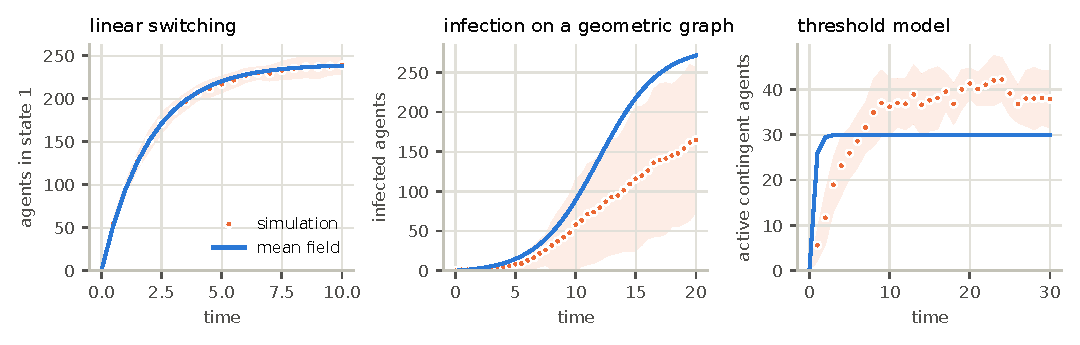
\includegraphics[width=\textwidth]{generated/fig-macro}
\caption{Automatically generated mean-field approximation (lines) and simulations (mean and $\pm 1$ standard deviation over seeds, markers and bands).
Left: 400 agents switching independently between two states (20 seeds).
Middle: infection with recovery on a random geometric graph of 1000 agents (10 seeds).
Right: number of active contingent agents in the threshold model of Fig.~\ref{fig:frames} (10 seeds).}
\label{fig:macro}
\end{figure*}
